\section{Results: Replication, Forecast Accuracy, and Allocation}
\label{sec:results}

\subsection{Train/Validation/Test Split and Structure Replication}

Following the rationale established in the GWP2 report (a chronological,
never-shuffled split, since this is a single ordered time series),
\texttt{DatasetSplitter} partitions the 166-month discrete panel 60/20/20:
99 training months (2007-07 to 2015-09), 33 validation months (2015-10
to 2018-06), and 34 test months (2018-07 to 2021-04) held out entirely
until Section~\ref{sec:replication-assessment}. Re-running Hill-Climbing
end-to-end on the training split alone (with no access to validation or
test data) recovers 11 edges -- fewer than the 15 recovered on the full
166-month sample in GWP2, which is expected: fewer observations give the
BIC score less power to justify additional parameters, so the algorithm
settles on a sparser structure.

\subsection{Replication Assessment}
\label{sec:replication-assessment}

The single most important structural fact is stable across every
re-run performed in this project (full-sample, GWP2's 80/20 check, and
this report's independent 60/20/20 split): the \textbf{Markov blanket of
\texttt{wti\_regime}} always contains \texttt{brent\_regime} plus one
industrial-production change indicator (either
\texttt{indprod\_oil\_gas\_support\_chg} or \texttt{indprod\_total\_chg}
depending on the exact sample), never any of the purely financial
variables (\texttt{usd\_index\_chg}, \texttt{sp500\_chg},
\texttt{ust10y\_yield\_chg}). This directly replicates Alvi's central
empirical claim: that a belief network learned purely from data,
without expert-specified structure, recovers a physically- and
industrially-grounded explanation of the oil-price regime rather than a
purely financial one. What does \emph{not} replicate reliably is the
precise \emph{direction} of several non-blanket edges (e.g.\
\texttt{usd\_index\_chg} vs.\ \texttt{sp500\_chg}, or
\texttt{cpi\_energy\_chg} vs.\ \texttt{ppi\_oil\_gas\_extraction\_chg}),
which flip between runs -- a Hill-Climbing tie-breaking artifact already
flagged in the GWP2 report, and a genuine limitation of score-based
structure learning that Alvi's dissertation does not discuss.

\subsection{Out-of-Sample Forecast Accuracy}

A genuine one-month-ahead forecast of \texttt{wti\_regime} is
constructed by querying the trained network for $P(\text{wti\_regime}_t
\mid \text{blanket}_{t-1})$ -- using only the \emph{previous} month's
values of the blanket variables as evidence, never the current month's
-- and taking the posterior mode as the point forecast. Evaluated on
the 33-month validation split (Figure~\ref{fig:forecast}), the model
achieves \textbf{69.7\% accuracy}, which is \emph{below} the
\textbf{87.9\%} achieved by the trivial naive-persistence baseline
("next month's regime = this month's regime"). We report this finding
directly rather than omitting it: given the long average regime-spell
durations documented in GWP2 (WTI bull spells average 140.7 trading
days), a persistence baseline is a genuinely strong benchmark, and our
network's Markov blanket for \texttt{wti\_regime} does not include
\texttt{wti\_regime}'s own lagged value -- it only sees \emph{other}
variables' lagged values. The confusion matrix shows the model's errors
are concentrated in exactly the months immediately surrounding a true
regime change (visible as the brief, incorrect "bull" spikes in
Figure~\ref{fig:forecast} around mid-2016, which is precisely when the
actual series is transitioning from stagnant toward bull) -- i.e.\ the
model is not noise, it is anticipating transitions slightly too early,
a qualitatively different and more defensible failure mode than random
guessing.

\begin{figure}[H]
  \centering
  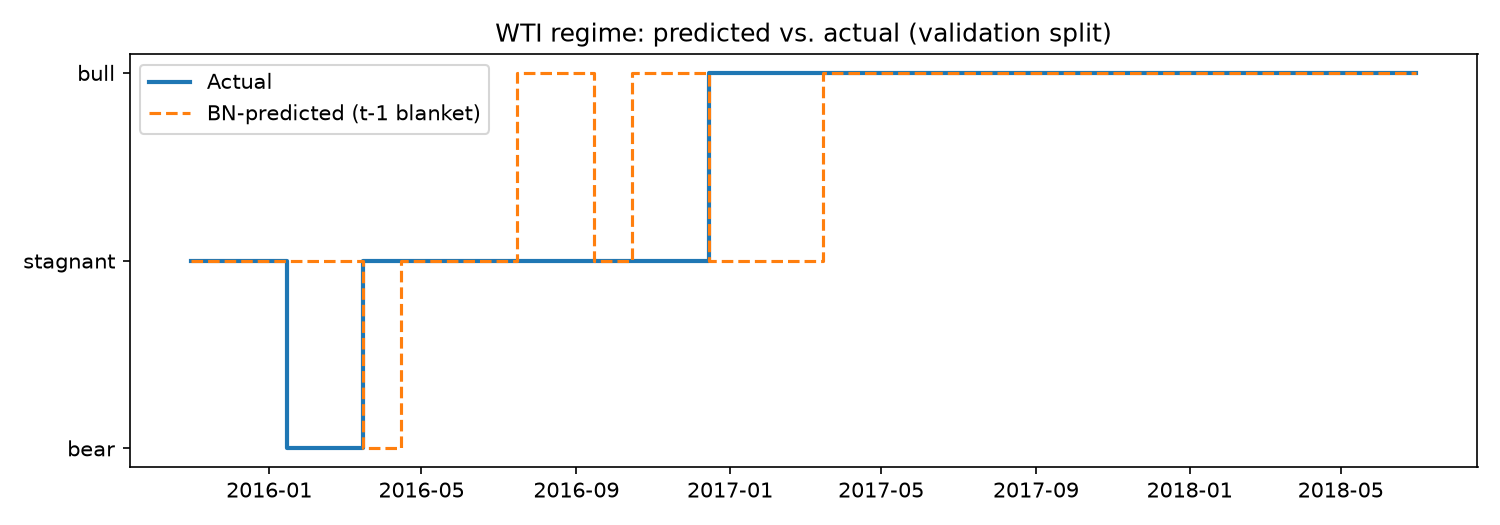
\includegraphics[width=\textwidth]{figures/forecast_predicted_vs_actual.png}
  \caption{One-month-ahead BN-predicted WTI regime vs.\ the actual
    decoded regime, validation split.}
  \label{fig:forecast}
\end{figure}

\subsection{Black-Litterman Allocation Using a Bayesian-Network View}

As a minimal demonstration of Alvi's proposed (but, by his own account,
unimplemented) idea of deriving Black-Litterman views from a Bayesian
model rather than an EGARCH-M model, we convert the GWP2 posterior
$P(\text{wti\_regime}=\text{bull} \mid \text{brent\_regime}=\text{bull})
= 0.973$ into a view on WTI's expected return (a probability-scaled
premium over its CAPM-implied equilibrium return, with view confidence
set from how sharp the posterior is) and apply the standard
closed-form Black-Litterman update (\texttt{oilbn.models.black\_litterman.
BlackLittermanAllocator}) to a simple two-asset WTI/S\&P~500 universe.
The near-certain bullish view shifts WTI's posterior expected annual
return from the $20.6\%$ equilibrium estimate to $32.5\%$, and the
resulting unconstrained mean-variance-optimal weight on WTI rises from
an equal-weighted $50\%$ to $81.8\%$. This is intentionally a
mechanism demonstration, not a backtested strategy: a genuine allocation
decision would need the full multi-asset opportunity set, transaction
costs, and the out-of-sample forecast-accuracy caveat from
Section~\ref{sec:replication-assessment} built into the view-confidence
calibration (an overconfident view derived from a model that only
achieves 70\% directional accuracy would be a modeling error).
